\documentclass[journal,12pt,twocolumn]{IEEEtran}
\usepackage{setspace}
\usepackage{gensymb}
\usepackage{xcolor}
\usepackage{caption}
\singlespacing
\usepackage{siunitx}
\usepackage[cmex10]{amsmath}
\usepackage{mathtools}
\usepackage{hyperref}
\usepackage{amsthm}
\usepackage{mathrsfs}
\usepackage{txfonts}
\usepackage{stfloats}
\usepackage{cite}
\usepackage{cases}
\usepackage{subfig}
\usepackage{longtable}
\usepackage{multirow}
\usepackage{enumitem}
\usepackage{bm}
\usepackage{mathtools}
\usepackage{listings}
\usepackage{tikz}
\usetikzlibrary{shapes,arrows,positioning}
\usepackage{circuitikz}
\renewcommand{\vec}[1]{\boldsymbol{\mathbf{#1}}}
\DeclareMathOperator*{\Res}{Res}
\renewcommand\thesection{\arabic{section}}
\renewcommand\thesubsection{\thesection.\arabic{subsection}}
\renewcommand\thesubsubsection{\thesubsection.\arabic{subsubsection}}

\renewcommand\thesectiondis{\arabic{section}}
\renewcommand\thesubsectiondis{\thesectiondis.\arabic{subsection}}
\renewcommand\thesubsubsectiondis{\thesubsectiondis.\arabic{subsubsection}}
\hyphenation{op-tical net-works semi-conduc-tor}

\lstset{
language=Python,
frame=single, 
breaklines=true,
columns=fullflexible
}
\begin{document}
\theoremstyle{definition}
\newtheorem{theorem}{Theorem}[section]
\newtheorem{problem}{Problem}
\newtheorem{proposition}{Proposition}[section]
\newtheorem{lemma}{Lemma}[section]
\newtheorem{corollary}[theorem]{Corollary}
\newtheorem{example}{Example}[section]
\newtheorem{definition}{Definition}[section]
\newcommand{\BEQA}{\begin{eqnarray}}
\newcommand{\EEQA}{\end{eqnarray}}
\newcommand{\define}{\stackrel{\triangle}{=}}
\newcommand{\myvec}[1]{\ensuremath{\begin{pmatrix}#1\end{pmatrix}}}
\newcommand{\mydet}[1]{\ensuremath{\begin{vmatrix}#1\end{vmatrix}}}
\bibliographystyle{IEEEtran}
\providecommand{\nCr}[2]{\,^{#1}C_{#2}} % nCr
\providecommand{\nPr}[2]{\,^{#1}P_{#2}} % nPr
\providecommand{\mbf}{\mathbf}
\providecommand{\pr}[1]{\ensuremath{\Pr\left(#1\right)}}
\providecommand{\qfunc}[1]{\ensuremath{Q\left(#1\right)}}
\providecommand{\sbrak}[1]{\ensuremath{{}\left[#1\right]}}
\providecommand{\lsbrak}[1]{\ensuremath{{}\left[#1\right.}}
\providecommand{\rsbrak}[1]{\ensuremath{{}\left.#1\right]}}
\providecommand{\brak}[1]{\ensuremath{\left(#1\right)}}
\providecommand{\lbrak}[1]{\ensuremath{\left(#1\right.}}
\providecommand{\rbrak}[1]{\ensuremath{\left.#1\right)}}
\providecommand{\cbrak}[1]{\ensuremath{\left\{#1\right\}}}
\providecommand{\lcbrak}[1]{\ensuremath{\left\{#1\right.}}
\providecommand{\rcbrak}[1]{\ensuremath{\left.#1\right\}}}
\theoremstyle{remark}
\newtheorem{rem}{Remark}
\newcommand{\sgn}{\mathop{\mathrm{sgn}}}
\newcommand{\rect}{\mathop{\mathrm{rect}}}
\newcommand{\sinc}{\mathop{\mathrm{sinc}}}
\providecommand{\abs}[1]{\left\vert#1\right\vert}
\providecommand{\res}[1]{\Res\displaylimits_{#1}} 
\providecommand{\norm}[1]{\left\Vert#1\right\Vert}
\providecommand{\mtx}[1]{\mathbf{#1}}
\providecommand{\mean}[1]{E\left[ #1 \right]}
\providecommand{\fourier}{\overset{\mathcal{F}}{ \rightleftharpoons}}
\providecommand{\ztrans}{\overset{\mathcal{Z}}{ \rightleftharpoons}}
\providecommand{\system}[1]{\overset{\mathcal{#1}}{ \longleftrightarrow}}
\newcommand{\solution}{\noindent \textbf{Solution: }}
\providecommand{\dec}[2]{\ensuremath{\overset{#1}{\underset{#2}{\gtrless}}}}
\let\StandardTheFigure\thefigure
\def\putbox#1#2#3{\makebox[0in][l]{\makebox[#1][l]{}\raisebox{\baselineskip}[0in][0in]{\raisebox{#2}[0in][0in]{#3}}}}
     \def\rightbox#1{\makebox[0in][r]{#1}}
     \def\centbox#1{\makebox[0in]{#1}}
     \def\topbox#1{\raisebox{-\baselineskip}[0in][0in]{#1}}
     \def\midbox#1{\raisebox{-0.5\baselineskip}[0in][0in]{#1}}

\vspace{3cm}
\title{Quadratic Programming Assignment}
\author{Gautam Singh}
\maketitle
\bigskip

\begin{abstract}
    This document contains the solution to Question 27 of Exercise 5 in Chapter
    6 of the class 12 NCERT textbook.
\end{abstract}

\begin{enumerate}
    \item The point on the curve 
    \begin{align}
        x^2 = 2y
        \label{eq:curve}
    \end{align}
    which is nearest to the point 
    $\vec{P} = \myvec{0\\5}$ is
    \begin{enumerate}
        \item $\myvec{2\sqrt{2}\\4}$
        \item $\myvec{2\sqrt{2}\\0}$
        \item $\myvec{0\\0}$
        \item $\myvec{2\\2}$
    \end{enumerate}

    \solution We need to find
    \begin{align}
        \min_{\vec{x}} g\brak{\vec{x}} &= \norm{\vec{x}-\vec{P}}^2 \label{eq:cost} \\
        \textrm{s.t. } h\brak{\vec{x}} &= \vec{x}^\top\vec{Vx} + 2\vec{u}^\top\vec{x} = 0 \label{eq:constr}
    \end{align}
    where
    \begin{align}
        \vec{V} = \myvec{1&0\\0&0},\ \vec{u} = \myvec{0\\-1}
    \end{align}
    First, we show that \eqref{eq:constr} is nonconvex. Indeed, suppose 
    $\vec{x_1}$ and $\vec{x_2}$ satisfy $h\brak{\vec{x}} = 0$. Then, 
    \begin{align}
        \vec{x_1}^\top\vec{Vx_1} + 2\vec{u}^\top\vec{x_1} + f &= 0 \label{eq:x1-parab} \\
        \vec{x_2}^\top\vec{Vx_2} + 2\vec{u}^\top\vec{x_2} + f &= 0 \label{eq:x2-parab}
    \end{align}
    Then, for any $0 \le \lambda \le 1$, substituting
    \begin{align}
        \vec{x_\lambda} \leftarrow \lambda\vec{x_1} + \brak{1-\lambda}\vec{x_2}
    \end{align}
    into \eqref{eq:constr}, we get
    \begin{align}
        h\brak{\vec{x_\lambda}} = \lambda\brak{\lambda-1}\brak{\vec{x_1}-\vec{x_2}}^\top\vec{V}\brak{\vec{x_1}-\vec{x_2}} + f \neq 0
        \label{eq:nonconvex}
    \end{align}
    Hence, the optimization problem is nonconvex. The constraints
    throw an error when \textit{cvxpy} is used, as shown in the erroneous Python code
    \texttt{codes/parab\_cvx.py}.

    We use the method of Lagrange multipliers instead to find the optima. Here, 
    we need to find $\lambda \in \mathbb{R}$ such that there exists a $\vec{x}$ 
    satisfying
    \begin{align}
        \nabla g\brak{\vec{x}} &= \lambda\nabla h\brak{\vec{x}} \\
        \implies 2\brak{\vec{x}-\vec{P}} &= 2\lambda\brak{\vec{Ax}+\vec{u}} \\
        \implies \brak{\vec{I}-\lambda\vec{A}}\vec{x} &= \lambda\vec{u} + \vec{P} \\
        \implies \myvec{1-\lambda&0\\0&1}\vec{x} &= \myvec{0\\5-\lambda}
        \label{eq:lagmul}
    \end{align}
    From \eqref{eq:lagmul}, we have two cases:
    \begin{enumerate}
        \item $\lambda \neq 1$. In this case, we form the augmented matrix
        \begin{align}
            \myvec{1-\lambda&0&0\\0&1&5-\lambda} \xleftrightarrow[]{R_1 \leftarrow \frac{R_1}{1-\lambda}} \myvec{1&0&0\\0&1&5-\lambda}
        \end{align}
        and get that
        \begin{align}
            \vec{x_m} = \myvec{0\\5-\lambda}
        \end{align}
        Substituting in \eqref{eq:constr} gives $\lambda = 5$. Thus, 
        $\vec{x_m} = \vec{0}$.

        \item $\lambda = 1$. In this case, \eqref{eq:lagmul} becomes
        \begin{align}
            \myvec{0&0\\0&1}\vec{x} &= \myvec{0\\4} \\
            \implies \vec{e_2}^\top\vec{x} = 4
            \label{eq:x-e2}
        \end{align}
        Substituting \eqref{eq:x-e2} into \eqref{eq:constr} becomes
        \begin{align}
            \brak{\vec{e_1}^\top\vec{x}}^2 &= 8 \\
            \implies \vec{e_1}^\top\vec{x} &= \pm 2\sqrt{2}
            \label{eq:x-e1}
        \end{align}
        Using \eqref{eq:x-e1} and \eqref{eq:x-e2},
        \begin{align}
            \vec{x_m} = \myvec{\pm 2\sqrt{2}\\4}
        \end{align}
    \end{enumerate}
    Using these values of $\vec{x_m}$, the distances are
    \begin{align}
        \norm{\myvec{0\\5}-\myvec{0\\0}} &= 5 \\
        \norm{\myvec{0\\5}-\myvec{\pm 2\sqrt{2}\\4}} &= 3
        \label{eq:true-min}
    \end{align}
    Thus, the correct answer is \textbf{a)}.

    We demonstrate both of the minima in \eqref{eq:true-min} is obtained using 
    constrained gradient descent in Fig. \ref{fig:gd-pits}, plotted using the 
    Python code \texttt{codes/grad\_pits.py}.
    \begin{figure}[!ht]
        \centering
        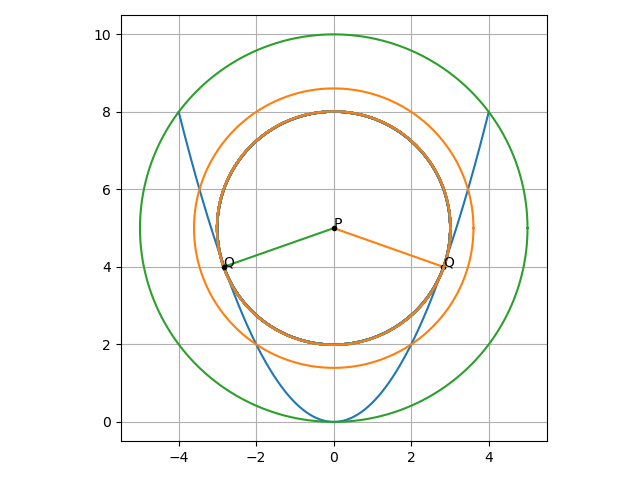
\includegraphics[width=\columnwidth]{figs/grad_pits.png}
        \caption{Gradient descent for a nonconvex optimization problem.}
        \label{fig:gd-pits}
    \end{figure}
\end{enumerate}
\end{document}
